We analyze the public 48-ns-holdoff measurements at optical densities 3 and 0, corresponding to low and high incident flux. Each acquisition supplies three disjoint segments of 20000 consecutive gaps: calibration, development and evaluation. The development segment exposes temporal clustering in low flux and motivates the additional transition component. Its form and the evaluation segment are fixed before fitting that component. Both fitting stages use calibration data only. Each segment retains its recorded timestamps.

A fixed-cutoff comparator estimates electronics recovery as the minimum calibration gap minus one raw timing-resolution unit (0.008 ns). It gives 77.745 ns in low flux and 76.809 ns in high flux. Each cutoff assigns zero density to one gap in its evaluation segment. Learning a single cutoff therefore leaves a short-gap prediction failure.

The variable-recovery and clustered-transition models assign finite density to all 40000 evaluation gaps. Their support contains all 10394778 gaps in the two complete acquisitions. Table~\ref{tab:measured} reports fitted parameters and evaluation results. The low-flux recovery scale reaches the 0.15-ns optimization bound; this segment does not resolve a narrower recovery distribution.

A cumulative distribution function (CDF) gives the fraction of gaps no longer than a specified duration. Its largest absolute prediction error summarizes the difference between measured and predicted gap distributions. Figure~\ref{fig:measured} uses 100000 next-gap predictions per model and acquisition, conditioned on the measured preceding phases. In low flux, the clustered-transition component reduces the whole-distribution CDF distance from 0.2449 to 0.0366 and improves mean log density by 0.7522 nats per transition. In high flux, its fitted fraction reaches the $10^{-6}$ lower bound; log density is unchanged to five decimal places, and CDF distances are 0.0310 and 0.0313. The extra component is useful for the low-flux clustering and adds no predictive gain in the high-flux segment.

\begin{table*}[t]\centering
\caption{Measured-data recovery and clustering fits. Each acquisition uses disjoint 20000-gap calibration, development and evaluation segments. Recovery location and scale are in ns. The fixed-cutoff column counts evaluation gaps assigned zero density by a cutoff estimated from the calibration minimum. Log-score gain is relative to recovery-only fitting, in nats per transition. CDF distances use the full evaluation gap range. At the cluster-fraction lower bound, the cluster time scale is not reported.}
\label{tab:measured}
\begin{tabular}{rrrrrrrrr}\toprule
OD & $\mu$ (ns) & $s_R$ (ns) & $q$ & $\pi$ & $\tau_b$ (ns) & \shortstack{Fixed-cutoff\\zero densities} & \shortstack{Log-score\\gain} & \shortstack{CDF distance\\recovery; mixture}\\\midrule
3 & 77.48 & 0.15 & 0.7607 & 0.2398 & 71.89 & 1 & +0.75220 & 0.2449; 0.0366\\
0 & 80.16 & 1.48 & 1.0000 & $10^{-6}$ & --- & 1 & 0.00000 & 0.0310; 0.0313\\
\bottomrule\end{tabular}\end{table*}

\begin{figure*}[t]\centering
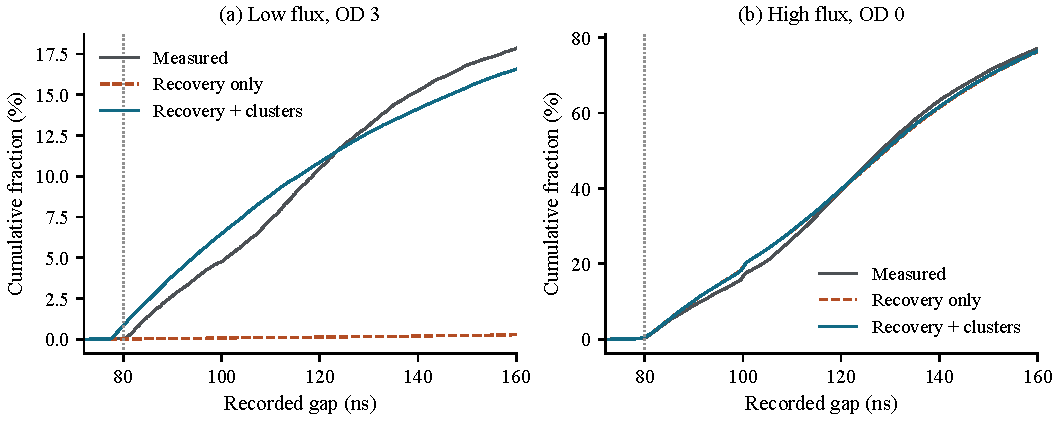
\includegraphics[width=\textwidth]{figures/fig06_measurements.pdf}
\caption{Measured gap distributions and calibrated transition-model predictions. Each empirical curve uses 20000 evaluation gaps disjoint from calibration and development. Each model curve uses 100000 next-gap predictions conditioned on the measured preceding phases. The displayed range emphasizes short gaps; reported CDF distances use the whole gap distribution. The dotted vertical line marks the nominal 80-ns electronics setting. In high flux the model predictions nearly coincide.}
\label{fig:measured}\end{figure*}
